\documentclass{article}
\usepackage[utf8]{inputenc}
\usepackage{graphicx}
\usepackage{appendix}

\title{C+A5}

\author{arcex012, mayxx394}
\date{October 29, 2018}

\begin{document}

\maketitle

\section{Experiments and Report}

\textbf{1.}
The metrics used in our experiment were the number of computation steps, the memory usage (max frontier count), and the time it took for each algorithm to run, timed with a python library called 'timeit'. 

For graph search used in Towers of Hanoi, we implemented 3 different ways of maintaining duplicate states that shouldn't be revisited. The first is a simple visited list, the second is an advanced visited list that takes node states back out if a node with lower depth is passed into the valid children function, and the third is a parent trace, checking parent nodes' states. Each of these implementations can be seen in the code pushed to GitHub. For our experiments we decided to use the simple visited list for all our algorithms, as the other two approaches were more time consuming.
\\*
\\*
\textbf{2.}
We chose to experiment with alpha, number of iterations, and starting value. Alpha was tested at 0.98 and 0.3 Number of iterations was tested at 500 and 2000 Starting value was tested at 600,000 and 10,000. End value was always 0.25
\\*
\\*
\textbf{3.}
The data collected was submitted on GitHub as text files while the tables and graphs are within an excel spreadsheet also uploaded to GitHub.
\\*
\\*
\textbf{4.}
Starting with Towers of Hanoi, the maximum problem size, n, that we could solve was:
\\*
\begin{itemize}
\item Dfs Graph: n = 11. When there were 12 towers present when we hit the 1 hour time limit. So only data for 11 towers was collected. 

\item Bfs Graph: n = 10. When there were 11 towers present when we hit the 1 hour time limit. So only data for 10 towers was collected. 

\item IDDfs Graph: n = 8. When there were 9 towers present when we hit the 1 hour time limit. So only data for 8 towers was collected. 

\end{itemize}
While for nQueens, the maximum problem size, n, that we could solve was: 
\begin{itemize}

\item Bfs Tree: n = 11. When there were 12 queens present on the 12 x 12 board, when we hit the 1 hour time limit. So only data for 11 queens was collected. 

\item IDDfs Tree: n = 11. When there were 12 queens present on the 12 x 12 board, when we hit the 1 hour time limit. So only data for 11 queens was collected. 

\item Simulated Annealing: n = 15 By setting alpha to 0.98, number of iterations to 2,000 start to 600,000 and end to 0.25 we were able to solve the 15 x 15 board 5 times in a row.
\end{itemize}
\newpage
\section{Graphs}
\begin{figure}[!htb]
\caption{Max Memory Usage - Towers of Hanoi}
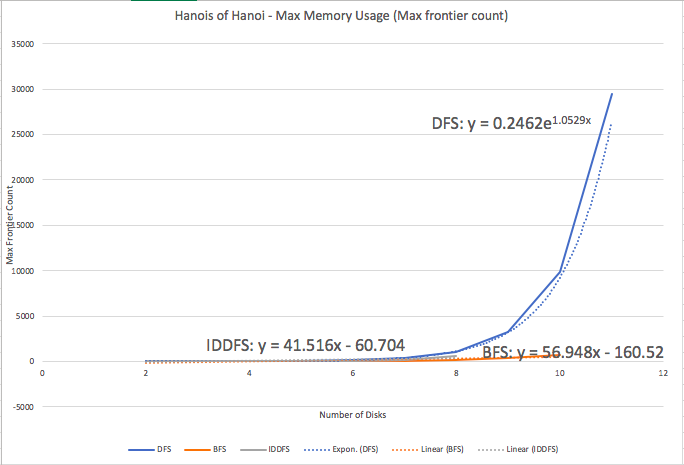
\includegraphics[width=\textwidth]{MemAll.png}
The above graph, Figure 1, shows that BFS has the lowest exponential factor which results in it using the least amount of memory as the number of discs increases.
\end{figure}

\begin{figure}[!htb]
\caption{Max Memory Usage - Towers of Hanoi}
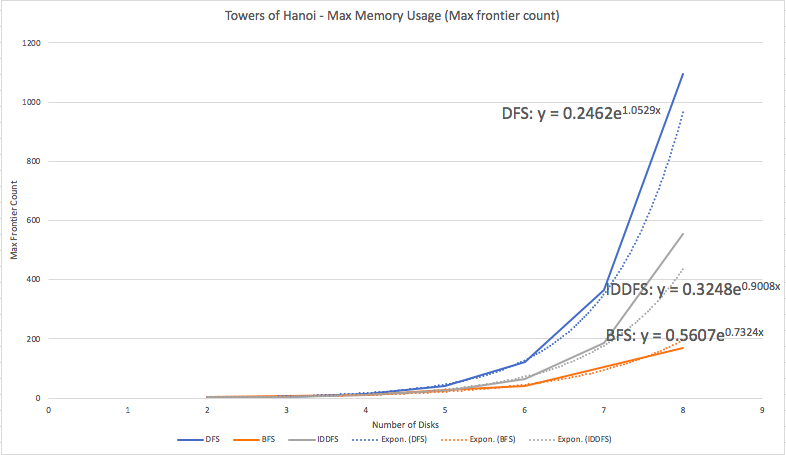
\includegraphics[width=\textwidth]{MemFew.png}
The above graph, Figure 2, is Figure 1 zoomed in. It shows that BFS has the lowest exponential factor which results in it using the least amount of memory as the number of discs increases.
\end{figure}

\begin{figure}[!htb]
\caption{Number of Steps Used - Towers of Hanoi}
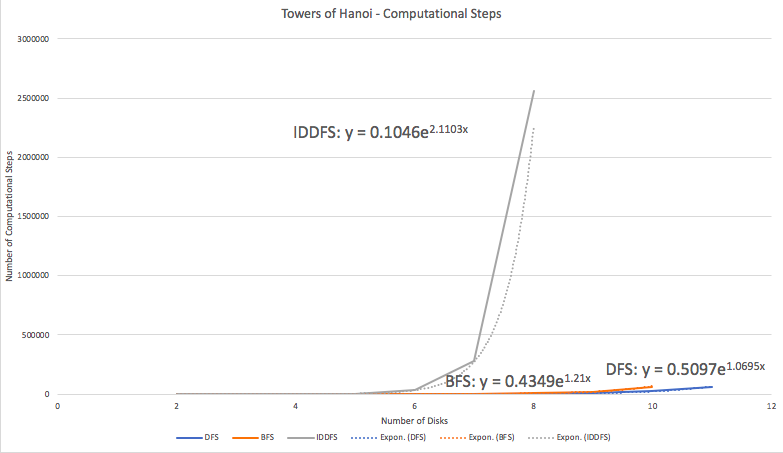
\includegraphics[width=\textwidth]{Steps.png}
In Figure 3, it is evident that IDDFS is the least efficient due to the huge spike in steps used, while BFS is the most efficient due to it having the smallest y value as x grows larger.
\end{figure}

\begin{figure}[!htb]
\caption{Time Taken - Towers of Hanoi}
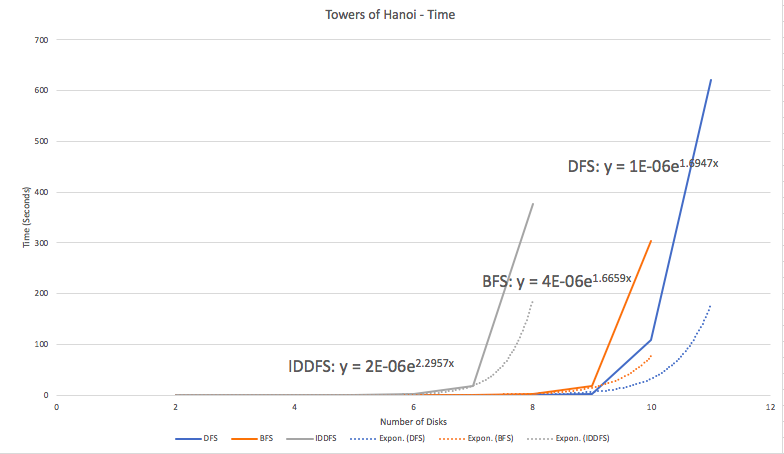
\includegraphics[width=\textwidth]{Time.png}
As seen in Figure 4, DFS performs faster than both the other algorithms, solving higher discs problems in less time.
\end{figure}

\begin{figure}[!htb]
\caption{Max Memory Usage - NQueens}
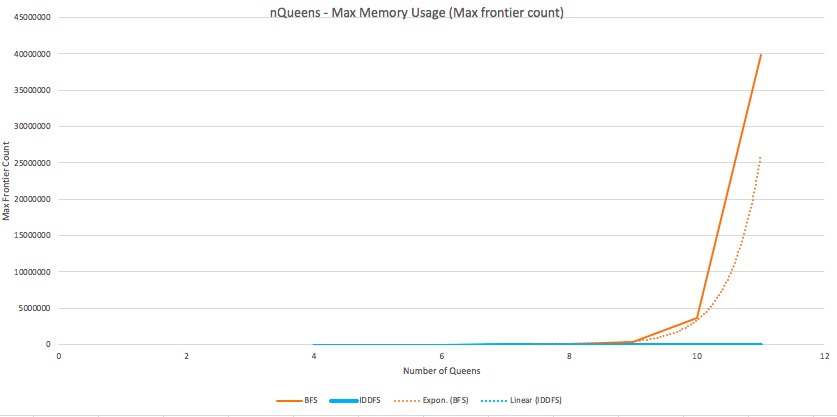
\includegraphics[width=\textwidth]{QMem.png}
In the above Figure 5, Bfs uses much more memory than IDDFS.
\end{figure}

\begin{figure}[!htb]
\caption{Average Steps for Simulated Annealing - NQueens 20}
Control = alpha:0.98 start:600,000 iterations:500
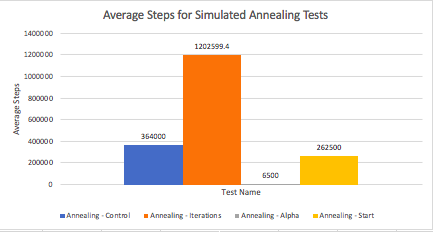
\includegraphics[width=\textwidth]{AvgSteps.png}
As depicted in Figure 6, annealing was the quickest with our low alpha value, and the slowest with our higher iterations value.
\end{figure}

\begin{figure}[!htb]
\caption{Average Value for Simulated Annealing - NQueens 20}
Control = alpha:0.98 start:600,000 iterations:500
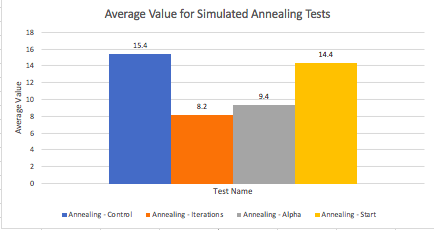
\includegraphics[width=\textwidth]{AvgValue.png}
Figure 7 shows that changing our iterations to 2,000 gave us the closest average state to the solution.
\end{figure}

\begin{figure}[!htb]
\caption{Highest Solvable Problem - NQueens 20}
Control = alpha:0.98 start:600,000 iterations:500
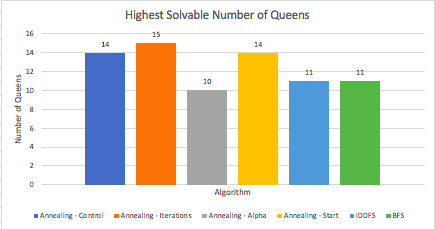
\includegraphics[width=\textwidth]{HighestSolve.png}
Figure 8 depicts that simulated annealing with a high iteration value let us solve larger NQueens problems than IDDFS and BFS.
\end{figure}

\clearpage


\section{Tables}

\begin{figure}[!htb]
\caption{NQueens Data for BFS and IDDFS}
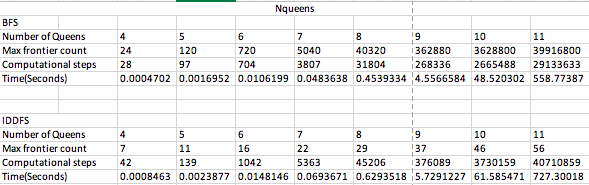
\includegraphics[width=\textwidth]{QueensComp.png}
Figure 9 shows our IDDFS Tree and BFS Tree data for NQueens. Computational steps and time go hand in hand, but both are displayed for reference. IDDFS has a much lower memory usage (max frontier count) than BFS, but is slightly slower.
\end{figure}

\begin{figure}[!htb]
\caption{Towers of Hanoi Data}
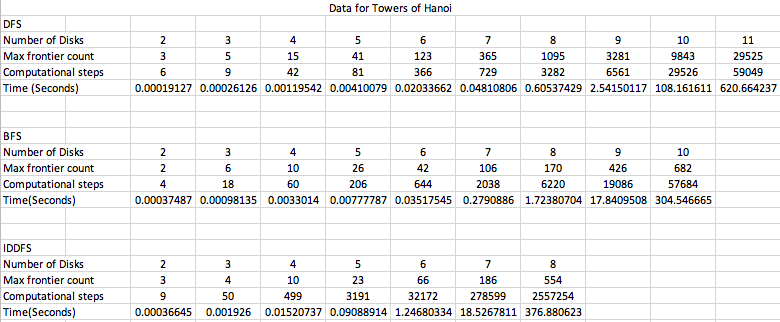
\includegraphics[width=\textwidth]{TowerTable.png}
Figure 10 shows the data for all our graph search algorithms. You can see that DFS runs the fastest, but also uses the most memory. BFS finds an optimal solution, but takes a significant while longer to run than DFS. IDDFS also finds the optimal solution, but runs slightly slower than BFS due to our visited list implementation.
\end{figure}


\begin{figure}[!htb]
\caption{Data From Simulated Annealing Testing for problem size 20}
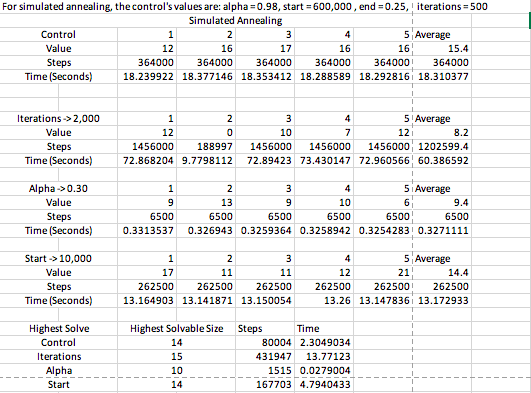
\includegraphics[width=\textwidth]{SimData.png}
In the above Figure 11, three different changes are compared to the initial control for simulated annealing, each ran on NQueens with size 20. Each has a different proficiency in value number of queens attacking each other(value), the number of steps taken, and the time it took to complete. Changing iterations to 2,000 gave us the lowest Value, with zero being the optimal solution. Changing alpha drastically reduced run time, and changing start reduced run time a little bit while giving us similar results to our control.
\end{figure}

\begin{figure}[!htb]
\caption{Comparison Results for Simulated Annealing}
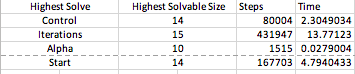
\includegraphics[width=\textwidth]{SimComp.png}
Figure 12 shows the highest size problem we can reliably solve 5 times in a row with each of our algorithms, and the time it takes to do so.
\end{figure}


\end{document}
